\documentclass[fleqn]{article}
\usepackage[utf8]{inputenc}
\usepackage{graphicx}
\usepackage{geometry}
\usepackage[fleqn]{amsmath}
\usepackage[export]{adjustbox}
\usepackage{tikz}
\usepackage{grffile}
\usepackage{hyperref}
\usepackage{epstopdf}
\usepackage{longtable}
\usepackage{subcaption}
\graphicspath{{/media/arul/envision/jan-may-2016/kernelmethods/Assignment-1/report/pics}}
\newgeometry{left=3cm, top=2cm, bottom=2cm}
\newcommand{\noimage}{%
  \setlength{\fboxsep}{-\fboxrule}%
  \fbox{\phantom{\rule{150pt}{100pt}}}% Framed box
}
\newcommand{\myparagraph}[1]{\paragraph{#1}\mbox{}\\}
\pagenumbering{gobble}
\setlength{\mathindent}{0pt}

\title{}
\author{Arulkumar S (CS15S023), Divya Saglani (CS15M041), Nitish (CS15S028)}

\date{$12^{th}$ May 2016}

\begin{document}
\setcounter{secnumdepth}{5}
\tracingall
\section{Introduction}
\section{Problem-1}
\newpage
\section{Support Vector Data Description (SVDD) (one class SVM)}

\subsection{Dataset - 3 (2-dimensional overlapping data)}

\subsubsection{Data}
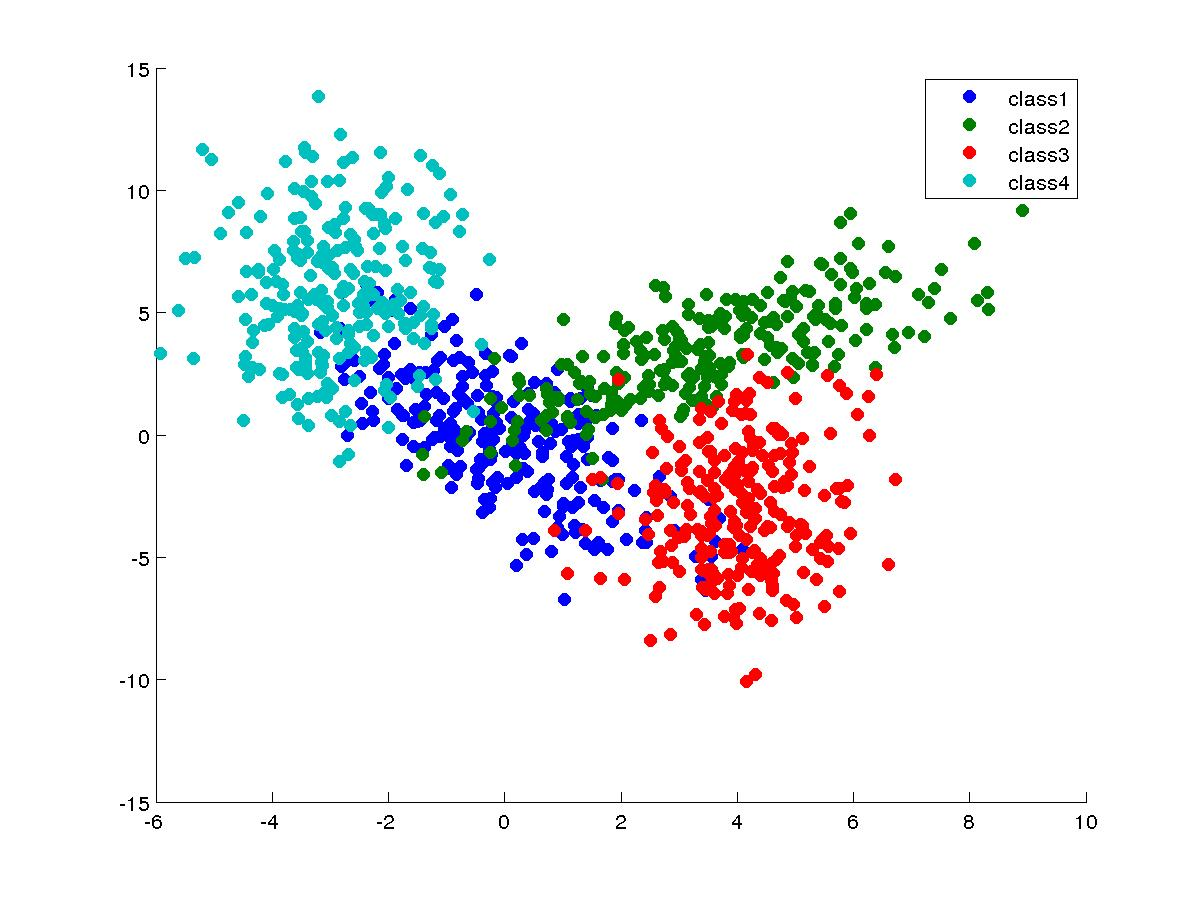
\includegraphics[scale=0.3]{./pics/dataset3_snap.jpg}\\\\
The class-1 data (plotted in Blue color) from the dataset-3 is selected as \\
'normal data' to be learned and represented by one-class SVM. 

\subsubsection{Procedure}
\begin{itemize}
  \item From the 2-dimensional overlapping data, one class (Class-1 with 250 data points) is selected as the 'normal' class used for training one class SVM.
  \item The data from other classes are uniformly sampled to form the validation (600 data points) and test set (400 data points), 
  which are used to verify the efficiency of the trained model.
  \item The one-class SVM (with $\nu$ as hyperparameter) classifier is trained using different $\nu$ values
   and the best model is choosen based on the performance in validation set. 
\end{itemize}

\subsubsection{Decision regions}
\myparagraph{Illustration: Almost-Hard-minimal hypersphere SVDD}

when $\nu = 0.01$, the SVDD model allows very less outliers. (i.e., Bounded support vectors = 1\% of the training data). \\
Hence, the model trained by having $\nu$ as 0.01 has the disadvantage of classifying all other class data which are included \
inside the hypersphere, as the 'Normal' class. This behaviour will affect the performance of classifier, as shown in the figure \ref{fig:nearhardmin}.

\begin{figure*}[t!]
    \centering
    \begin{subfigure}[t]{0.5\textwidth}
        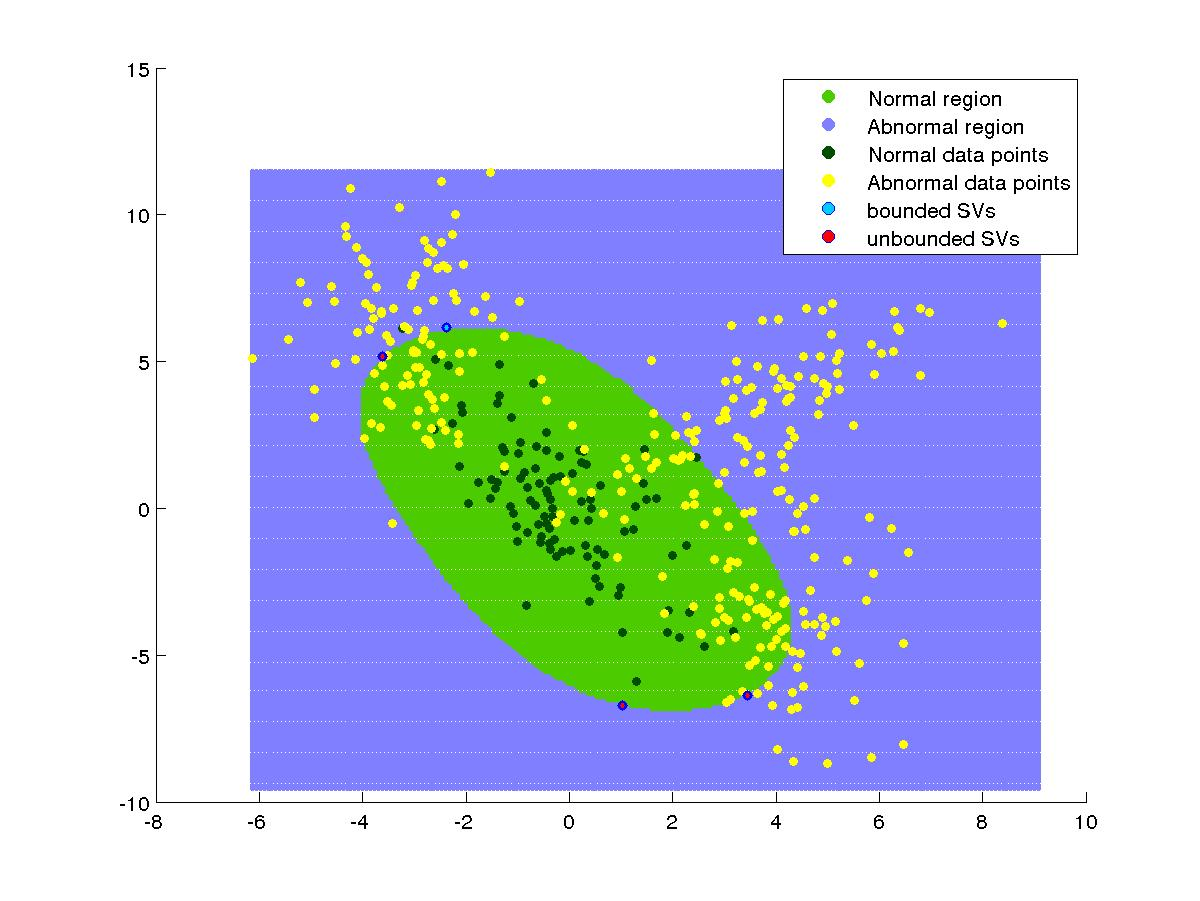
\includegraphics[scale=0.3, left]{./pics/task2_decisionregion_g=0.01_n=0.01.jpg}
        \caption{One-class SVM with RBF kernel (gamma = 0.01, $\nu$ = 0.01, bounded SVs = 1, unbounded SVs = 3)}
    \end{subfigure}
    \begin{subfigure}[t]{0.5\textwidth}
        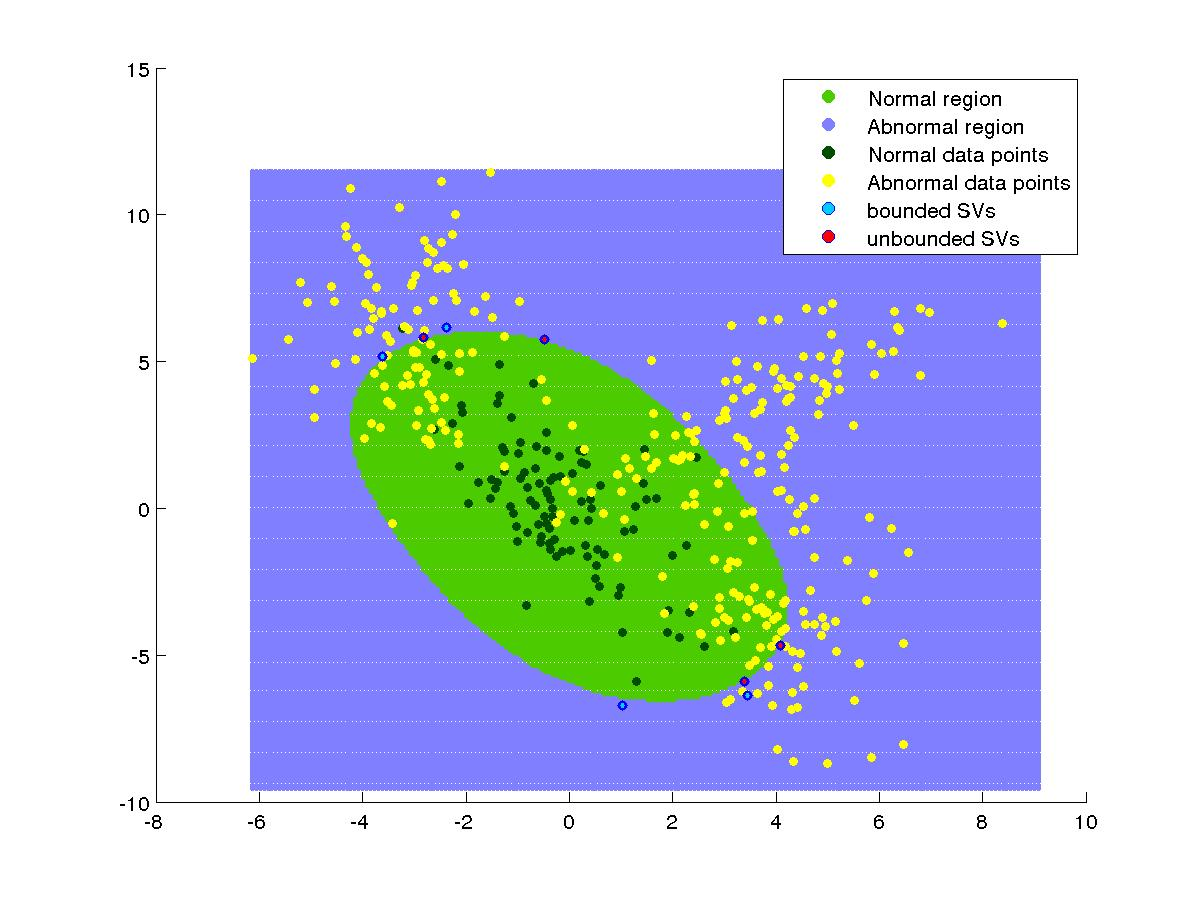
\includegraphics[scale=0.3, left]{./pics/task2_decisionregion_g=0.01_n=0.02.jpg}
        \caption{One-class SVM with RBF kernel (gamma = 0.01, $\nu$ = 0.02, bounded SVs = 4, unbounded SVs = 4)}
    \end{subfigure}
    \caption{illustration of Almost-hard-minimal hypersphere which gives poor performance\label{fig:nearhardmin}}
\end{figure*}

\newpage
\myparagraph{Confusion matrices \& performance details}

\subparagraph{$\nu$ = 0.01, RBF kernel parameter ($\gamma$) = 0.01}
~\\\\
\textbf{Validation data}\\

\begin{center}
  \begin{longtable}{ c | c | c  }
	\multicolumn{1}{c}{ } & 
	\multicolumn{1}{c}{Abnormal class (predicted)} & 
	\multicolumn{1}{c}{Normal class (predicted)} \\
    \hline
    Abnormal class (Target)& 289 & 161 \\ \hline
    Normal class (Target)&  4 & 146 \\ \hline
  \end{longtable}
\end{center}    

\begin{center}
  \begin{longtable}{ c | c | c  }
  	\multicolumn{1}{c}{ } & 
	\multicolumn{1}{c}{Formula} & 
	\multicolumn{1}{c}{Value} \\\hline
	True positive rate w.r.t., Normal class (recall)  & $\frac{TP}{TP + FN}$ & 0.973 \\\hline
	False positive rate w.r.t., Normal class (fall-out)  & $\frac{FP}{TN + FP}$ & 0.357\\\hline
	F1-score & $\frac{2TP}{2TP + FN + FP}$ & 0.638\\\hline
	Accuracy  & & 68.75\%\\\hline
  \end{longtable}
\end{center} 


~\\
\textbf{Test data}\\

\begin{center}
  \begin{longtable}{ c | c | c  }
	\multicolumn{1}{c}{ } & 
	\multicolumn{1}{c}{Abnormal class (predicted)} & 
	\multicolumn{1}{c}{Normal class (predicted)} \\
    \hline
    Abnormal class (Target)& 176 & 124 \\ \hline
    Normal class (Target)&  1 & 99 \\ \hline
  \end{longtable}
\end{center}    

\begin{center}
  \begin{longtable}{ c | c | c }
  	\multicolumn{1}{c}{ } & 
	\multicolumn{1}{c}{Formula} & 
	\multicolumn{1}{c}{Value} \\\hline
	True positive rate w.r.t., Normal class (recall)  & $\frac{TP}{TP + FN}$ & 0.999 \\\hline
	False positive rate w.r.t., Normal class (fall-out)  & $\frac{FP}{TN + FP}$ & 0.413\\\hline
	F1-score & $\frac{2TP}{2TP + FN + FP}$ & 0.613\\\hline
	Accuracy & & 68.75\%\\\hline
  \end{longtable}
\end{center} 

\subparagraph{$\nu$ = 0.02, RBF kernel parameter ($\gamma$) = 0.01}
~\\\\
\textbf{Validation data}\\

\begin{center}
  \begin{longtable}{ c | c | c  }
	\multicolumn{1}{c}{ } & 
	\multicolumn{1}{c}{Abnormal class (predicted)} & 
	\multicolumn{1}{c}{Normal class (predicted)} \\
    \hline
    Abnormal class (Target)& 285 & 163 \\ \hline
    Normal class (Target)&  5 & 145 \\ \hline
  \end{longtable}
\end{center}    

\begin{center}
  \begin{longtable}{ c | c | c  }
  	\multicolumn{1}{c}{ } & 
	\multicolumn{1}{c}{Formula} & 
	\multicolumn{1}{c}{Value} \\\hline
	True positive rate w.r.t., Normal class (recall)  & $\frac{TP}{TP + FN}$ & 0.966 \\\hline
	False positive rate w.r.t., Normal class (fall-out)  & $\frac{FP}{TN + FP}$ & 0.362\\\hline
	F1-score & $\frac{2TP}{2TP + FN + FP}$ & 0.632\\\hline
	Accuracy  & & 68.5\%\\\hline
  \end{longtable}
\end{center} 


~\\
\textbf{Test data}\\

\begin{center}
  \begin{longtable}{ c | c | c  }
	\multicolumn{1}{c}{ } & 
	\multicolumn{1}{c}{Abnormal class (predicted)} & 
	\multicolumn{1}{c}{Normal class (predicted)} \\
    \hline
    Abnormal class (Target)& 175 & 125 \\ \hline
    Normal class (Target)&  1 & 99 \\ \hline
  \end{longtable}
\end{center}    

\begin{center}
  \begin{longtable}{ c | c | c  }
  	\multicolumn{1}{c}{ } & 
	\multicolumn{1}{c}{Formula} & 
	\multicolumn{1}{c}{Value} \\\hline
	True positive rate w.r.t., Normal class (recall)  & $\frac{TP}{TP + FN}$ & 0.99 \\\hline
	False positive rate w.r.t., Normal class (fall-out)  & $\frac{FP}{TN + FP}$ & 0.417\\\hline
	F1-score & $\frac{2TP}{2TP + FN + FP}$ & 0.611\\\hline
	Accuracy & & 68.75\%\\\hline
  \end{longtable}
\end{center} 

\myparagraph{Soft-minimal hypersphere for better performance}
To get an optimal soft-minimal hypersphere, $\nu$ can be set as 0.1 or 0.2 to allow 10\% or 20\%
outliers (Bounded support vectors) of the data to lie out of the minimal hypersphere. This will give higher performance, as it will reduce the misclassification rate, as shown in the figure \ref{fig:softminsphere}.

\begin{figure*}[t!]
    \centering
 	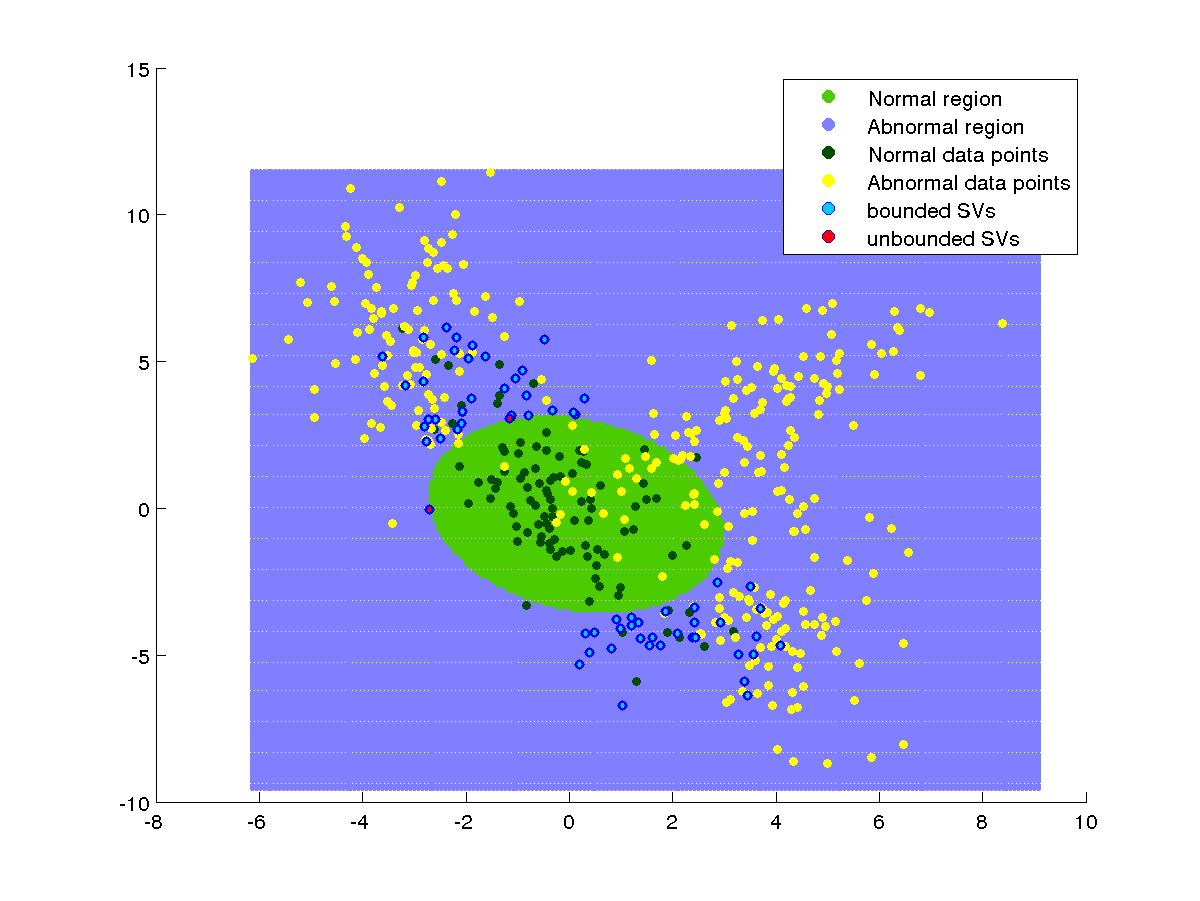
\includegraphics[scale=0.3]{./pics/task2_decisionregion_g=0.01_n=0.25.jpg}
     \caption{illustration of optimal soft-minimal hypersphere which gives good performance\label{fig:softminsphere}.
     One-class SVM with RBF kernel (gamma = 0.01, $\nu$ = 0.25, bounded SVs = 61, unbounded SVs = 2)}
\end{figure*}

\subparagraph{$\nu$ = 0.25, RBF kernel parameter ($\gamma$) = 0.01}
~\\\\
\textbf{Validation data}\\

\begin{center}
  \begin{longtable}{ c | c | c  }
	\multicolumn{1}{c}{ } & 
	\multicolumn{1}{c}{Abnormal class (predicted)} & 
	\multicolumn{1}{c}{Normal class (predicted)} \\
    \hline
    Abnormal class (Target)& 408 & 42 \\ \hline
    Normal class (Target)&  31 & 119 \\ \hline
  \end{longtable}
\end{center}    

\begin{center}
  \begin{longtable}{ c | c | c  }
  	\multicolumn{1}{c}{ } & 
	\multicolumn{1}{c}{Formula} & 
	\multicolumn{1}{c}{Value} \\\hline
	True positive rate w.r.t., Normal class (recall)  & $\frac{TP}{TP + FN}$ & 0.793 \\\hline
	False positive rate w.r.t., Normal class (fall-out)  & $\frac{FP}{TN + FP}$ & 0.0933\\\hline
	F1-score & $\frac{2TP}{2TP + FN + FP}$ & 0.765\\\hline
	Accuracy  & & 87.83\%\\\hline
  \end{longtable}
\end{center} 


~\\
\textbf{Test data}\\

\begin{center}
  \begin{longtable}{ c | c | c  }
	\multicolumn{1}{c}{ } & 
	\multicolumn{1}{c}{Abnormal class (predicted)} & 
	\multicolumn{1}{c}{Normal class (predicted)} \\
    \hline
    Abnormal class (Target)& 269 & 31 \\ \hline
    Normal class (Target)& 22 & 78 \\ \hline
  \end{longtable}
\end{center}    

\begin{center}
  \begin{longtable}{ c | c | c  }
  	\multicolumn{1}{c}{ } & 
	\multicolumn{1}{c}{Formula} & 
	\multicolumn{1}{c}{Value} \\\hline
	True positive rate w.r.t., Normal class (recall)  & $\frac{TP}{TP + FN}$ & 0.78 \\\hline
	False positive rate w.r.t., Normal class (fall-out)  & $\frac{FP}{TN + FP}$ & 0.103\\\hline
	F1-score & $\frac{2TP}{2TP + FN + FP}$ & 0.746\\\hline
	Accuracy & & 86.75\%\\\hline
  \end{longtable}
\end{center} 

\subsection{Dataset-4 : Breast benign}
\subsubsection{Procedure}
\begin{itemize}
  \item The given normal data (458 data points) is splitted into 70\% as training set, 10\% as validation set, the remaining 20\% as test set.
  \item The given abnormal data (241 data points) is split into 50\% as validation set and 50\% as test set.
  \item One-class SVM (with RBF kernel) is trained only with Normal Data and the hyper-parameter($\nu$) is fixed using validation set.
  \item The efficiency of chosen model is evaluated using test set and results are reported.  
\end{itemize}

\newpage
The best validation performance of 94.54\% is obtained, when RBF kernel parameter ($\gamma$) = 0.001 and $\nu$ = 0.05,
with Bounded SVs = 13, unbounded SVs = 4.

\subsection{Confusion matrices and performance details}

\subsubsection{Validation data}

\begin{center}
  \begin{longtable}{ c | c | c  }
	\multicolumn{1}{c}{ } & 
	\multicolumn{1}{c}{Abnormal class (predicted)} & 
	\multicolumn{1}{c}{Normal class (predicted)} \\
    \hline
    Abnormal class (Target)& 116 & 4 \\ \hline
    Normal class (Target)&  5 & 40 \\ \hline
  \end{longtable}
\end{center}    

\begin{center}
  \begin{longtable}{ c | c | c  }
  	\multicolumn{1}{c}{ } & 
	\multicolumn{1}{c}{Formula} & 
	\multicolumn{1}{c}{Value} \\\hline
	True positive rate w.r.t., Normal class (recall)  & $\frac{TP}{TP + FN}$ & 0.889 \\\hline
	False positive rate w.r.t., Normal class (fall-out)  & $\frac{FP}{TN + FP}$ & 0.0334\\\hline
	F1-score & $\frac{2TP}{2TP + FN + FP}$ & 0.898\\\hline
	Accuracy  & & 94.54\%\\\hline
  \end{longtable}
\end{center} 


\subsubsection{Test data}

\begin{center}
  \begin{longtable}{ c | c | c  }
	\multicolumn{1}{c}{ } & 
	\multicolumn{1}{c}{Abnormal class (predicted)} & 
	\multicolumn{1}{c}{Normal class (predicted)} \\
    \hline
    Abnormal class (Target)& 118 & 3 \\ \hline
    Normal class (Target)& 4 & 89 \\ \hline
  \end{longtable}
\end{center}    

\begin{center}
  \begin{longtable}{ c | c | c  }
  	\multicolumn{1}{c}{ } & 
	\multicolumn{1}{c}{Formula} & 
	\multicolumn{1}{c}{Value} \\\hline
	True positive rate w.r.t., Normal class (recall)  & $\frac{TP}{TP + FN}$ & 0.956 \\\hline
	False positive rate w.r.t., Normal class (fall-out)  & $\frac{FP}{TN + FP}$ & 0.025\\\hline
	F1-score & $\frac{2TP}{2TP + FN + FP}$ & 0.962\\\hline
	Accuracy & & 96.72\%\\\hline
  \end{longtable}
\end{center} 

\newpage
\section{Problem-3}
\section{Problem-4}
\newpage
\section{Problem-5 : Structured data classification}
\subsection{Task}
The chosen task is to perform ``classification'' on Graphs for 
activity against non-small cell lung cancer and ovarian cancer cell lines.

\subsection{Dataset}

\begin{itemize}
  \item The dataset NCI1 represent two balanced subsets of data sets of chemical compounds screened 
for activity against non-small cell lung cancer and ovarian cancer cell lines respectively
(Wale and Karypis (2006) and \url{http://pubchem.ncbi.nlm.nih.gov}). 
  \item The dataset contain 4110 instances of chemical compound activities represented as Graphs.
  \item The dataset is splitted into 70\% as Training data, 10\% as Validation data, 20\% as Test data.
\end{itemize}

\subsection{Kernel}
We use one of the graph kernel from Weisfeiler-Lehman (WL) Kernels family to define the similarity
between two graphs. The kernel is called as ``WL shortest path kernel''. In essence, the shortest 
path kernel counts pairs of shortest paths with the same distance between identically labeled 
source and sink nodes on the original graphs.

All of the Weisfeiler-Lehman (WL) Kernels for given two graphs G, G' consists of basic 4 steps. as below:\\

Let the graphs be G, G', as shown in the picture.\\
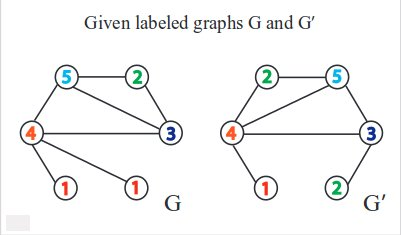
\includegraphics[scale=0.4]{./pics/twographs.jpg}

\begin{itemize}
  \item \textbf{Multiset-label determination} : assign a multiset-label to each node in G and G' which consists of the multiset of neighborhood nodes.
  \item \textbf{Sorting each multiset} :  Sort elements in the Multiset-label and concatenate them into a string.\\
  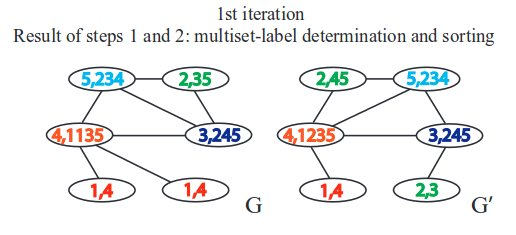
\includegraphics[scale=0.4]{./pics/labelsfindingandsorting.jpg}
  \item \textbf{Label compression} : Sort all of the strings for all $v \in G \& G'$ in ascending order. Map each distinct string into a new label
  	using function $f: \sum^* \rightarrow \sum$, where $f(string(v)) = f(string(w))$, iff, $string(v) = string(w)$\\
  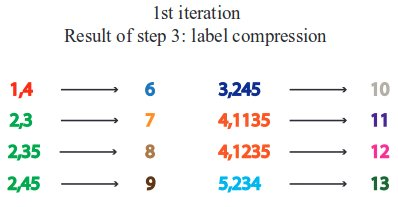
\includegraphics[scale=0.4]{./pics/compression.jpg}
  \item \textbf{Relabeling} : for all nodes in graphs G, G', set the label as $f(string(v))$\\
  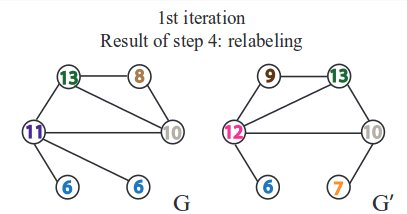
\includegraphics[scale=0.4]{./pics/relabeling.jpg}
  
\end{itemize}

These four steps are repeated to get a final relabeled graph from which the Kernel's feature maps are derived.

\myparagraph{Base kernel}

we consider the base kernel $k_{SP}$ of the form $k_{SP}$(G, G') = $\phi_{SP}(G)^T\phi_{SP}(G')$, where $\phi_{SP}(G)^T$ is a vector whose components are number of occurences of triplets of the form
$<a, b, p>$ in G, where a,b $\in \sum$ are ordered end-point labels of shortest path and  p $\in N_0 $ is the shortest path length.  
The base kernel at each iteration i, can be combined together to give out the final kernel.

$k_{WLshortestpath}^{h} = k_{SP}(G_0, G'_0) + k_{SP}(G_1, G'_1) + \dots + k_{SP}(G_h, G'_h)$  

\subsection{Confusion matrices and performance details}

For the current dataset (NCI1), the iteration count is set as 3. The base kernel matrices for all the three iterations are retrieved and 
added to get the actual kernel $k_{WLshortestpath}^{h}$.

The best performance is achieved with $\nu$ = 0.3. In the best model, the number of bounded SVs = 422, number of unbounded SVs = 1255.

\subsubsection{Validation data}

\begin{center}
  \begin{longtable}{ c | c | c  }
	\multicolumn{1}{c}{ } & 
	\multicolumn{1}{c}{non-small cell lung cancer (predicted)} & 
	\multicolumn{1}{c}{ovarian cancer cell (predicted)} \\
    \hline
    non-small cell lung cancer (Target)& 181 & 24 \\ \hline
    ovarian cancer cell (Target)&  30 & 175 \\ \hline
  \end{longtable}
\end{center}    

\begin{center}
  \begin{longtable}{ c | c | c  }
  	\multicolumn{1}{c}{ } & 
	\multicolumn{1}{c}{Formula} & 
	\multicolumn{1}{c}{Value} \\\hline
	True positive rate w.r.t., Normal class (recall)  & $\frac{TP}{TP + FN}$ & 0.854 \\\hline
	False positive rate w.r.t., Normal class (fall-out)  & $\frac{FP}{TN + FP}$ & 0.218\\\hline
	F1-score & $\frac{2TP}{2TP + FN + FP}$ & 0.866\\\hline
	Accuracy  & & 86.82\%\\\hline
  \end{longtable}
\end{center} 


\subsubsection{Test data}

\begin{center}
  \begin{longtable}{ c | c | c  }
	\multicolumn{1}{c}{ } & 
	\multicolumn{1}{c}{non-small cell lung cancer (predicted)} & 
	\multicolumn{1}{c}{ovarian cancer cell (predicted)} \\
    \hline
    non-small cell lung cancer (Target)& 338 & 75 \\ \hline
    ovarian cancer cell (Target)&  54 & 357 \\ \hline
  \end{longtable}
\end{center}    

\begin{center}
  \begin{longtable}{ c | c | c  }
  	\multicolumn{1}{c}{ } & 
	\multicolumn{1}{c}{Formula} & 
	\multicolumn{1}{c}{Value} \\\hline
	True positive rate w.r.t., Normal class (recall)  & $\frac{TP}{TP + FN}$ & 0.868 \\\hline
	False positive rate w.r.t., Normal class (fall-out)  & $\frac{FP}{TN + FP}$ & 0.291\\\hline
	F1-score & $\frac{2TP}{2TP + FN + FP}$ & 0.846\\\hline
	Accuracy  & & 84.34\%\\\hline
  \end{longtable}
\end{center} 

\end{document}